\section{Konzept zur Modulimplementierung für die Verhaltensklassifizierung} \label{sec:Meth FinalKonzept}
Durch die Erkenntnisse, Konzepte und Methoden lässt sich das Modul aus \autoref{sec:Meth gesamtkonzept} konkretisieren. In \autoref{sec:Meth Nutzwert} erfolgt die Eingrenzung auf einfache Modelle des überwachten Lernens. Daraus geht die Erkenntnis hervor, dass  die Zeitreihen der Ereignisse komprimiert werden müssen, damit das Modell Sequenzen verstehen kann. In \autoref{sec:Meth Datensatz} wird erläutert, dass ein festes Intervall für die zuverlässige Anwendung des Moduls notwendig ist. In \autoref{sec:Meth FeatExtr} wird die notwendige Vorverarbeitung der Rohdaten weiter aufgeschlüsselt. Es wird der Weg von den Rohdaten zu einem Featurevektor aufgezeigt. Anschließend ist in \autoref{sec:Meth FeatHypModSelect} erläutert wie sich die Featureauswahl ergibt, wie das beste Modell erwählt wird und wie dieses einzustellen ist, um die beste Performance zu erhalten. Danach erfolgt die Fertigstellung des Modells durch das Training und den finalen Test mit dem Testdatensatz. Um den Machine Learning Worflow abzuschließen, wird das Modell in die Anwendung, das Modul, integriert. Dadurch ergibt sich das in \autoref{fig:ModulFinalKOnzept} abgebildete Blockschaltbild für das Modul zur Verhaltensklassifikation.


\begin{figure}[htb]
    \centering
    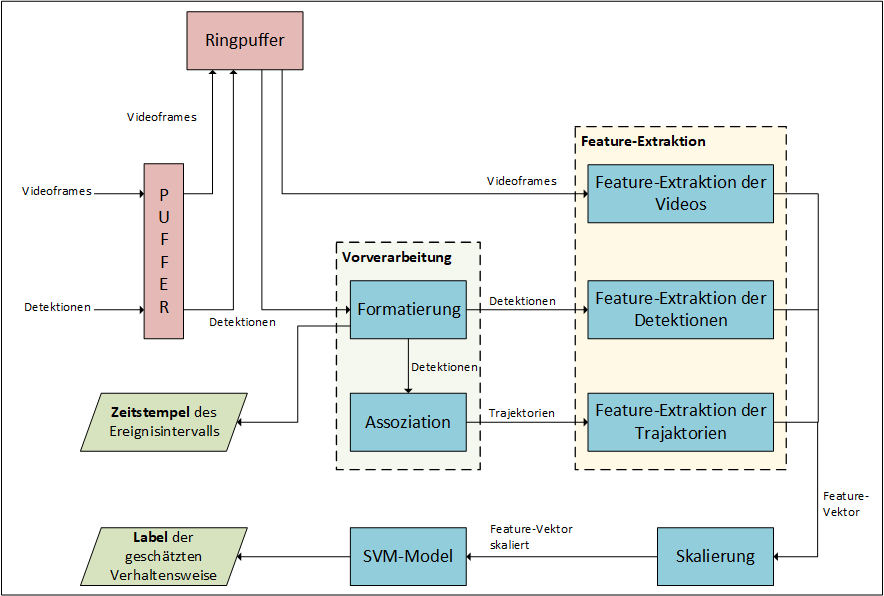
\includegraphics[width=\textwidth]{img/Grafiken/Gesamtkonzept Final.png}
    \caption[Finales Konzept für das Modul zur Verhaltensklassifikation.]{Finales Konzept für das Modul zur Verhaltensklassifikation.}
    \label{fig:ModulFinalKOnzept}
\end{figure}


Zu sehen ist die Vorverarbeitung aus der Feature-Extraktion bestehend aus dem Formatieren  der Detektionsdaten und dem Generieren der Trajektorien. Auch die Feature-Extraktion ist so implementiert wie in \autoref{sec:Meth FeatExtr}, jedoch sind die einzelnen Komponenten an die Feature-Auswahl aus \autoref{sec:Meth FeatHypModSelect} angepasst. Als Modell wird die trainierte und eingestellte polynomiale SVM integriert. Für eine optimale Anwendung der SVM wird der Featurevektor auf einen Wertebereich von [-1;1] skaliert. Die Skalierung bezieht sich auf die Features im Trainingsdatensatz. Damit unbekannte Ereignisse korrekt geschätzt werden können, muss die Skalierungsinformation während des Modellaufbaus gespeichert werden. Anschließend wird die Skalierung in das Modul integriert. Das Modell schätzt die Zugehörigkeit zu einer Verhaltensweise und gibt das entsprechende Label aus.\par

Der Pufferspeicher ist bereits in \autoref{sec:Meth gesamtkonzept} zu sehen. Er dient dazu, die Rohdaten zwischenzuspeichern, während sie auf die Verarbeitung warten. Er funktioniert nach dem First In-First Out (\acrshort{FIFO}) Prinzip \cite{Sedgewick.2011}. Während das Modul ein Ereignis verarbeitet, werden im Puffer neu eintreffende Daten abgelegt. Bisher unerwähnt ist der Ereignisspeicher des Moduls. In diesem liegen die Rohdaten zu dem Ereignis, das aktuell verarbeitet wird. Neben dem Puffer wird ein zweiter Speicher benötigt, um eine lückenlose Abtastung des Stallgeschehens zu erreichen. Im Idealfall entsteht eine Überlappung mit den Intervallen, wodurch ein Ereignis zuverlässig und so früh wie möglich erkannt werden kann. \par

Die Aufgabe des Ereignisspeichers ist am besten an einem Beispiel zu beschreiben. Die Auswertung wird gestartet. Zu Beginn liegen keine Rohdaten vor. Der Puffer und der Ereignisspeicher sind leer. Nun treffen neue Rohdaten im Puffer ein. Das Modul ist mit keiner Verarbeitung beschäftigt, deshalb zieht es die Rohdaten direkt in den Ereignisspeicher. Dieser Ereignisspeicher wird abgefragt, ob er bereits Rohdaten für ein Intervall von 40 Sekunden hat. Solange dies nicht der Fall ist, werden die Daten aus dem Puffer in den Ereignisspeicher geschoben. Sobald genügend Rohdaten für ein Intervall im Ereignisspeicher vorliegen, werden die Verarbeitung und die Schätzung gestartet. Ab diesem Moment werden die Rohdaten aus dem Puffer nicht mehr in den Ereignisspeicher überführt. Ist die Auswertung des Intervalls abgeschlossen, wird ermittelt, welche Dauer die Rohdaten im Puffer umfassen. Im Beispiel sind das 10 Sekunden. Diese neusten 10 Sekunden im Puffer überschreiben die ältesten 10 Sekunden im Ereignisspeicher. Dort liegen sofort genug Rohdaten für das nächste Intervall vor und die Auswertung wird wieder gestartet. Die ausgewerteten Intervalle sind im Beispiel um 10 Sekunden verschoben. Dadurch entsteht eine Überlappung von 30 Sekunden. Das Stallgeschehen wird lückenlos abgetastet. \par

Der Ereignisspeicher steht in einer Analogie zu Ringpufferspeichern. Bei diesem werden die ältesten Daten mit den neusten überschrieben. Somit befinden sich im Ereignisspeicher immer Daten zu einem Zeitraum von maximal 40 Sekunden. Dabei ist wichtig klarzustellen, dass bei einer Verarbeitung die Daten nicht aus dem Ereignisspeicher gelöscht werden, da diese für die nächste Verarbeitung teilweise wieder verwendet werden. Die Abfrage erfolgt bei einem Ringpufferspeicher ebenfalls nach dem \acrshort{FIFO} Prinzip, wodurch die zeitliche Reihenfolge der Daten bewahrt wird \cite{Sedgewick.2011}.\par

Durch diesen Aufbau ergibt sich eine Abtastrate des Moduls, die ungefähr der Verarbeitungszeit der Auswertung entspricht. Eine genau Aufschlüsselung der Laufzeiten folgt in \autoref{sec:Ergeb Sim}. \par

Der Pufferspeicher wird als eine \gls{IMDB} realisiert. \gls{IMDB}[s] sind Datenbanken, die im Arbeitsspeicher eines Rechners aufgebaut sind. Klassische Datenbanken befinden sich in der Regel auf Festplatten. Durch die Platzierung im Arbeitsspeicher werden sehr schnelle Zugriffszeiten ermöglicht. Arbeitsspeicher ist deutlich teurer als Festplattenspeicher, weswegen i. d. R. deutlich weniger davon zur Verfügung steht. Das Modul hat keine kritischen Anforderungen an die Arbeitsspeichermenge. Die benötigte Speichermenge ist für moderne Rechner problemlos zu realisieren. \par


\subsection{Simulation der Anwendung des Moduls} \label{sec:Meth Sim}
Da die Aufzeichnungen im Putenmaststall vor Beginn der Arbeit bereits abgeschlossen waren, gibt es keine Möglichkeit, das Modul im Feld zu testen. Stattdessen wird ein Konzept entwickelt, mit dem die Anwendung simuliert werden kann. Da die Trainingsdaten aus einer sehr überschaubaren Datenmenge stammen, wie in \autoref{sec:Meth Datensatz} dargestellt, steht eine große Anzahl an unbekannten Daten zur Verfügung. Diese können für eine Simulation verwendet werden. \par

Simuliert werden soll die Anwendung des Moduls auf einen ganzen Tag. Die Aufzeichnungen fanden während der Mastdurchläufe täglich von 5:00 Uhr morgens bis 22:20 Uhr abends statt. Das Modul soll einen vollen Tag, mit Rohdaten aus 17 Stunden und 20 Minuten, verarbeiten und die Verhaltensweisen des Stallgeschehens schätzen.\par

Dazu wird ein Detektionsdatensatz benötigt, das die Daten eines ganzen Tages umfasst. Ebenfalls ist das dazugehörige Video herauszusuchen. Video und Detektionsdatensatz werden eingelesen. Der Detektionsdatensatz wird Eintrag für Eintrag chronologisch in die \gls{IMDB} des Puffers geschoben. Vorher wird das Frame aus dem Video ermittelt, das zu dem Eintrag passt. Dieses wird ebenfalls in den Puffer geschoben. Eine Zeitverzögerung ist einzubauen, die die Framerate simuliert. Die tatsächliche mittlere Framerate der Aufzeichnung lässt sich aus dem Detektionsdatensatz bestimmen. Diese wird genutzt, um die Zeitverzögerung einzustellen. So wird der Rohdatenstrom des Moduleingangs simuliert. Das Modul verarbeitet den Datenstrom und gibt die geschätzten Verhaltensweisen als Labels zurück. Diese werden zusammen mit dem Start- und Endzeitpunkt des jeweiligen Intervalls für die Auswertung abgespeichert. Das Blockdiagramm in der Abbildung \ref{fig:ModulKonzeptSim} zeigt das Konzept zur Simulation. 

\begin{figure}[htb]
    \centering
    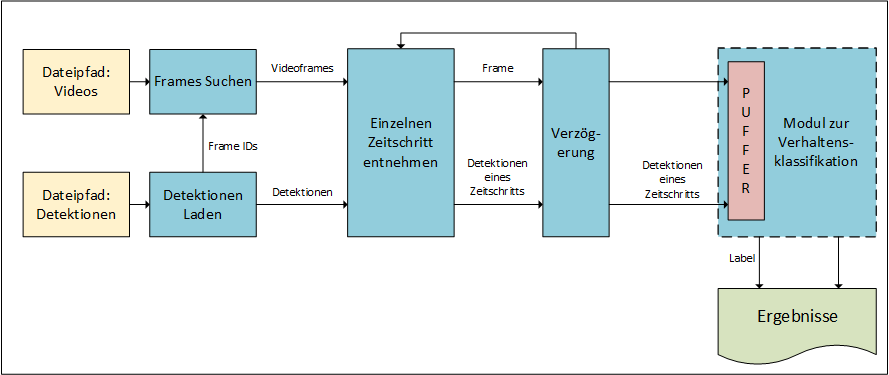
\includegraphics[width=\textwidth]{img/Grafiken/Konzept Simultaion.png}
    \caption[Konzept zur Simulation der Anwendung des Moduls zur Verhaltensklassifikation.]{Konzept zur Simulation der Anwendung des Moduls zur Verhaltensklassifikation.}
    \label{fig:ModulKonzeptSim}
\end{figure}

Mit der Simulation sollen folgende Punkte ermittelt werden:

\begin{itemize}
    \item \textbf{Auslegung des Puffers:} Der benötigte Speicherplatz für die \gls{IMDB} soll bestimmt werden.
    \item \textbf{Laufzeiten:} Die Laufzeiten des Moduls und seiner Komponenten sind zu messen.
    \item \textbf{Abtastrate}: Die genaue Abtastrate des Moduls soll bestimmt werden. Das ist über die Laufzeiten möglich.
    \item \textbf{Latenz:} Ermittelt werden soll die maximale Latenz zwischen dem Startpunkt eines Ereignisses und dem Vorliegen des Ergebnisses der Schätzung.
    \item \textbf{Echtzeitfähigkeit:} Am Ende ist zu beurteilen, ob das Modul als echtzeitfähig einzustufen ist.
\end{itemize}
